\documentclass[twoside]{book}

% Packages required by doxygen
\usepackage{fixltx2e}
\usepackage{calc}
\usepackage{doxygen}
\usepackage[export]{adjustbox} % also loads graphicx
\usepackage{graphicx}
\usepackage[utf8]{inputenc}
\usepackage{makeidx}
\usepackage{multicol}
\usepackage{multirow}
\PassOptionsToPackage{warn}{textcomp}
\usepackage{textcomp}
\usepackage[nointegrals]{wasysym}
\usepackage[table]{xcolor}

% Font selection
\usepackage[T1]{fontenc}
\usepackage[scaled=.90]{helvet}
\usepackage{courier}
\usepackage{amssymb}
\usepackage{sectsty}
\renewcommand{\familydefault}{\sfdefault}
\allsectionsfont{%
  \fontseries{bc}\selectfont%
  \color{darkgray}%
}
\renewcommand{\DoxyLabelFont}{%
  \fontseries{bc}\selectfont%
  \color{darkgray}%
}
\newcommand{\+}{\discretionary{\mbox{\scriptsize$\hookleftarrow$}}{}{}}

% Page & text layout
\usepackage{geometry}
\geometry{%
  a4paper,%
  top=2.5cm,%
  bottom=2.5cm,%
  left=2.5cm,%
  right=2.5cm%
}
\tolerance=750
\hfuzz=15pt
\hbadness=750
\setlength{\emergencystretch}{15pt}
\setlength{\parindent}{0cm}
\setlength{\parskip}{3ex plus 2ex minus 2ex}
\makeatletter
\renewcommand{\paragraph}{%
  \@startsection{paragraph}{4}{0ex}{-1.0ex}{1.0ex}{%
    \normalfont\normalsize\bfseries\SS@parafont%
  }%
}
\renewcommand{\subparagraph}{%
  \@startsection{subparagraph}{5}{0ex}{-1.0ex}{1.0ex}{%
    \normalfont\normalsize\bfseries\SS@subparafont%
  }%
}
\makeatother

% Headers & footers
\usepackage{fancyhdr}
\pagestyle{fancyplain}
\fancyhead[LE]{\fancyplain{}{\bfseries\thepage}}
\fancyhead[CE]{\fancyplain{}{}}
\fancyhead[RE]{\fancyplain{}{\bfseries\leftmark}}
\fancyhead[LO]{\fancyplain{}{\bfseries\rightmark}}
\fancyhead[CO]{\fancyplain{}{}}
\fancyhead[RO]{\fancyplain{}{\bfseries\thepage}}
\fancyfoot[LE]{\fancyplain{}{}}
\fancyfoot[CE]{\fancyplain{}{}}
\fancyfoot[RE]{\fancyplain{}{\bfseries\scriptsize Generated by Doxygen }}
\fancyfoot[LO]{\fancyplain{}{\bfseries\scriptsize Generated by Doxygen }}
\fancyfoot[CO]{\fancyplain{}{}}
\fancyfoot[RO]{\fancyplain{}{}}
\renewcommand{\footrulewidth}{0.4pt}
\renewcommand{\chaptermark}[1]{%
  \markboth{#1}{}%
}
\renewcommand{\sectionmark}[1]{%
  \markright{\thesection\ #1}%
}

% Indices & bibliography
\usepackage{natbib}
\usepackage[titles]{tocloft}
\setcounter{tocdepth}{3}
\setcounter{secnumdepth}{5}
\makeindex

% Custom commands
\newcommand{\clearemptydoublepage}{%
  \newpage{\pagestyle{empty}\cleardoublepage}%
}

\usepackage{caption}
\captionsetup{labelsep=space,justification=centering,font={bf},singlelinecheck=off,skip=4pt,position=top}

%===== C O N T E N T S =====

\begin{document}

% Titlepage & ToC
\pagenumbering{roman}
\begin{titlepage}
\vspace*{7cm}
\begin{center}%
{\Large N\+E24 Homework }\\
\vspace*{1cm}
{\large Generated by Doxygen 1.8.11}\\
\end{center}
\end{titlepage}
\clearemptydoublepage
\tableofcontents
\clearemptydoublepage
\pagenumbering{arabic}

%--- Begin generated contents ---
\chapter{Documentation}
\label{md_documentation}
{\bfseries Derived from material by Anthony Scopatz}

Just like version control and testing, documenting your code is the {\bfseries most important thing} you can do as a software developer. Good documentation is a sublime experience that should permeate your code.

Documentation is important because it is {\tt the only way that 90\% of people will ever interact with you or your code}. In fact, it is the only way that scales up; there are only so many emails that you can (and want) write.

What is disturbing is that documentation is a forgotten after thought for most developers. It turns out that being able to write software {\itshape and} being able to write in your primary spoken language are {\itshape different skills}. Luckily, we are academics so it is in our nature to publish / write. We have no excuse for bad documentation.

\subsection*{The Many Stages of Documentation}


\begin{DoxyEnumerate}
\item Code Comments
\item A\+PI Documentation
\item Auto-\/\+Documentation
\item Self-\/\+Documenting Code
\item Readmes
\item User Guides
\item Developer Guides
\end{DoxyEnumerate}

\subsection*{Code Comments}

Every language has a special character (or two) that indicate(s) to the parser, compiler, or interpreter that whatever comes after or between these characters should be ignored. This allows the author to write, annotate, and explain the code that they are writing {\itshape right at the point that they are writing it!} This is especially helpful if something weird, obtuse, or obscure is about to happen because it gives the author a chance to explain themselves to future developers (often themselves in 1, 2, 6, etc. months).

The best part is that you can put literally {\itshape anything} in comments\+: publication citations, A\+S\+C\+II art, messages to your friends, and threats to your collaborators.

In Python, the comment character is the hash symbol {\ttfamily \#}. The following example shows how you might help explain a toaster\+:

\begin{DoxyVerb}def toast(slices, toastiness, msg=None):

    # make sure the toaster has the right setting
    toastiness = int(toastiness) if 0 < toastiness else 5

    print "Engage the bread warming!"
    for slice in slices:
        slice.toast(toastiness)

    # log the message, making a default if needed
    if msg is None:
        msg = "Toasted to level {}".format(toastiness)
    logging.info(msg)
\end{DoxyVerb}


However, it is certainly possible to over-\/document your code with comments. Comments should never simply repeat what the code itself is doing. The goal is to strike the right balance. The appropriate ratio changes with language. (Typically higher level languages have greater functionality per line and so have more comments per amount of code.) Try to avoid the following\+:

\begin{DoxyVerb}# init a to 0
a = 0

# make b 'a string'
b = 'a string'

# Add one to a
a = a + 1

# stopping excessive comments
self.fall_on_sword()
\end{DoxyVerb}


Note\+: my personal tendency is to over-\/comment. It doesn\textquotesingle{}t necessarily hurt anything, but what might some detractors be?

\subsection*{A\+PI Documentation}

The application programming interface (A\+PI) is the definition of the protocol that two pieces of code may use to interact with one another. Consider the case of functions. All functions have a function signature that specifies how many arguments they accept and their return values. This signature, along with the module name and function name, is the A\+PI. (The function object/pointer itself is the implementation and is independent of the abstract A\+PI.)

Just because you have an argument list, however, does not imply that the meaning of the arguments is known. For example\+:

\begin{DoxyVerb}def f(a, b=10):

    # ...
    return
\end{DoxyVerb}


We know that {\ttfamily f()} accepts two argument {\ttfamily a} and {\ttfamily b} and that {\ttfamily b} should probably be an integer. But what does {\ttfamily f()} actually do? What do these arguments mean in this context?

Python allows the user to define A\+PI documentation right at the function, class, module, or variable definition. Every Python object may have a {\ttfamily \+\_\+\+\_\+doc\+\_\+\+\_\+} attribute that is a string representation of the A\+PI docs. This is known as a {\itshape docstring}. {\tt P\+E\+P257} describes the conventions for docstrings. The most important of these is that simple things should have simple docstrings.

If, right below a definition, in the first non-\/comment, non-\/whitespace line, there is an unassigned string literal, then this string is automatically loaded as the docstring. It is this docstring that is then read by the {\ttfamily help()} built-\/in or the {\ttfamily ?} in i\+Python.

\begin{DoxyVerb}def mean(numlist):
    """Computes the mean of a list of numbers."""

    try:
        total = sum(numlist)
        length = len(numlist)
    except ValueError:
        print "The number list was not a list of numbers."
    except:
        print "There was a problem evaluating the number list."
    return total/length


def fib(n):
    """Determines the nth Fibonacci number, where n is 
    a non-negative integer."""

    if n < 0 or int(n) != n:
        return NotImplemented
    elif n == 0 or n == 1:
        return n
    else:
        return fib(n - 1) + fib(n - 2)

print help(mean)
print fib.__doc__
\end{DoxyVerb}


Most Python docstrings are written in a markup language called {\tt re\+Structured\+Text} (r\+ST). It is designed to be easy to read, extensible, and provide enough natural-\/looking syntax to be able to render nicely. For example, our toaster docstring might look like\+:

\begin{DoxyVerb}def toast(slices, toastiness, msg=None):
    """Toast some bread.

    Parameters
    ----------
    slices : sequence of instance of bread slices
        Toast slices to toastiness level
    toastiness : int
        The desired toaster setting
    msg : str, optional
        A message for the toaster's usage log.

    """

    # make sure the toaster has the right setting
    toastiness = int(toastiness) if 0 < toastiness else 5

    print "Engage the bread warming!"
    for slice if slices:
        slice.toast(toastiness)

    # log the message, making a default if needed
    if msg is None:
        msg = "Toasted to level {}".format(toastiness)
    logging.info(msg)
\end{DoxyVerb}


\subsection*{Auto-\/\+Documentation}

Automatic documentation is the powerful concept that the comments and docstrings that the developer has already written can be scraped from the code base and placed on a website or into A\+PI documentation. This significantly reduces the overhead of having to write and maintain many documents that contain effectively the same information.

Probably the three most popular auto-\/doc projects are {\tt javadoc} for Java, {\tt Doxygen} for most compiled languages, and {\tt sphinx} for Python.

{\bfseries Example\+:} Let\textquotesingle{}s try to make some documentation using Doxygen and the example file {\tt {\ttfamily multilevel\+\_\+solver.\+py}}.

\subsection*{Exercise}

You can build the Doxygen documentation by making a stub Doxygen file for your python code. We\textquotesingle{}re going to do this for the {\tt {\ttfamily Jelly\+Bean\+Code}} \begin{DoxyVerb} doxygen -g doc_example
\end{DoxyVerb}


Now you have a Doxygen template called doc\+\_\+example. Open the doc\+\_\+example file. There are many entries you can edit. The ones we\textquotesingle{}re going to worry about here\+:

1) Let\textquotesingle{}s change the project name \begin{DoxyVerb} PROJECT_NAME           = "Jelly Bean Code"
\end{DoxyVerb}


2) Tell Doxygen what files to use \begin{DoxyVerb} INPUT                  =  "EstNumJellies.py"
\end{DoxyVerb}


3) Tell it to optimize for Python \begin{DoxyVerb} OPTIMIZE_OUTPUT_JAVA   = YES
\end{DoxyVerb}


Information about formatting Doxygen comments for Python can be found {\tt here}.

Let\textquotesingle{}s build what we\textquotesingle{}ve got now and check it out \begin{DoxyVerb} doxygen doc_example
 cd html
 google-chrome index.html
\end{DoxyVerb}


Add some additional Doxygen formatted comments to the functions in the {\ttfamily Est\+Num\+Jellies.\+py} module. Then, using Doxygen, generate a website that auto-\/documents this module.

Feel free to peruse the multilevel\+\_\+solver.\+py code for a more complicated example.

\subsection*{Self-\/\+Documenting Code}

Much like in testing where you can simply write perfect code the first time, there is an analogous philosophy is documentation. This is the philosophy of {\tt self-\/documenting code}. This ethos makes the claim that it is often possible to write code in such a way that new readers can understand what the code does simply by reading it. Therefore, no extra documentation is required. It is all there in the code itself.

While there are obvious pitfalls with this approach (assumed knowledge on the reader\textquotesingle{}s behalf, unavoidable complexities, etc.) there are some merits. By having meaningful naming conventions and structure it does become possible to infer a lot about a code just by glancing at it. Coding standards come from the same desire to have readable software.

However, using this documentation strategy exclusively is {\itshape highly} inadvisable.

\subsection*{Readmes}

The omnipresent {\ttfamily R\+E\+A\+D\+ME} file is typically a plain text file that sits next to the code. They may contain markup, but are often quite terse. point of a readme file is to provide only the most basic information to the user / developer.

Readme files are so common that Git\+Hub will render and display the readme file for all directories whenever you are browsing a source tree. Even Linux itself has a {\tt readme}\+:

\begin{quote}
Linux kernel release 3.\+x {\tt http\+://kernel.\+org/}

These are the release notes for Linux version 3. Read them carefully, as they tell you what this is all about, explain how to install the kernel, and what to do if something goes wrong.

W\+H\+AT IS L\+I\+N\+UX?

Linux is a clone of the operating system Unix, written from scratch by Linus Torvalds with assistance from a loosely-\/knit team of hackers across the Net. It aims towards P\+O\+S\+IX and Single U\+N\+IX Specification compliance.

It has all the features you would expect in a modern fully-\/fledged Unix, including true multitasking, virtual memory, shared libraries, demand loading, shared copy-\/on-\/write executables, proper memory management, and multistack networking including I\+Pv4 and I\+Pv6.

It is distributed under the G\+NU General Public License -\/ see the accompanying C\+O\+P\+Y\+I\+NG file for more details.

... \end{quote}


\subsection*{User Guides}

The next level of documentation are user guides. These often take the form of books or pdfs that aim to explain top level architecture and functionality to (possibly novice) users. Such documents are extremely helpful for bringing in new users, helping existing users learn more complex features, going in depth into the theory (math, biology, physics, chemistry, engineering), and as a reference manual for advanced users and developers. However, because of their high level nature, you typically have to wait until the code has stabilized to be able to write a good, comprehensive user\textquotesingle{}s guide.

{\bfseries Examples\+:} {\tt F\+L\+A\+SH}, {\tt Num\+Py}.

\subsection*{Developer Guides}

Developer guides are very similar to user guides, except that they assume a basic mastery of the project. They are typically for people who want to {\itshape become} developers on a project rather than for existing developers. They are probably most important for code projects that have plugin architectures and/or where the line between user and developer is less well defined.

{\bfseries Examples\+:} {\tt Android}, {\tt Python}. 
\chapter{homework question}
\label{md_homework_question}
NE 24 Homework \#3 Gerardo Alvarado 4/11/16 \section*{Assignment 7 }

{\tt https\+://developer.\+chrome.\+com/extensions/devguide}

The Google Chrome developer guide provides a basic, concise guide for what Chrome is M\+E\+A\+NT to do, describing key features of the application, while also giving useful information for programming and improving the application. 
\chapter{NE 24}
\label{md_README}
List of things contained in this folder\+:


\begin{DoxyEnumerate}
\item Two functions are located in this folder. a. Est\+Num\+Jellies.\+py -\/ calculates the number of jellybeans in the world using input data. b. multilevel\+\_\+solver.\+py
\item One example input for the Est\+Num\+Jellies.\+py function
\item Documentation files
\item A Homework folder containing the doxygen homework build. 
\end{DoxyEnumerate}
\chapter{Hierarchical Index}
\section{Class Hierarchy}
This inheritance list is sorted roughly, but not completely, alphabetically\+:\begin{DoxyCompactList}
\item \contentsline{section}{Est\+Num\+Jellies.\+Num\+Jelly\+Estimator}{\pageref{class_est_num_jellies_1_1_num_jelly_estimator}}{}
\item object\begin{DoxyCompactList}
\item \contentsline{section}{multilevel\+\_\+solver.\+Grid}{\pageref{classmultilevel__solver_1_1_grid}}{}
\item \contentsline{section}{multilevel\+\_\+solver.\+Grid\+Set}{\pageref{classmultilevel__solver_1_1_grid_set}}{}
\end{DoxyCompactList}
\end{DoxyCompactList}

\chapter{Class Index}
\section{Class List}
Here are the classes, structs, unions and interfaces with brief descriptions\+:\begin{DoxyCompactList}
\item\contentsline{section}{{\bf multilevel\+\_\+solver.\+Grid} }{\pageref{classmultilevel__solver_1_1_grid}}{}
\item\contentsline{section}{{\bf multilevel\+\_\+solver.\+Grid\+Set} }{\pageref{classmultilevel__solver_1_1_grid_set}}{}
\item\contentsline{section}{{\bf Est\+Num\+Jellies.\+Num\+Jelly\+Estimator} \\*This class estimates the number of jelly beans in the world using input data determined to be correlated to this result }{\pageref{class_est_num_jellies_1_1_num_jelly_estimator}}{}
\end{DoxyCompactList}

\chapter{Class Documentation}
\section{multilevel\+\_\+solver.\+Grid Class Reference}
\label{classmultilevel__solver_1_1_grid}\index{multilevel\+\_\+solver.\+Grid@{multilevel\+\_\+solver.\+Grid}}
Inheritance diagram for multilevel\+\_\+solver.\+Grid\+:\begin{figure}[H]
\begin{center}
\leavevmode
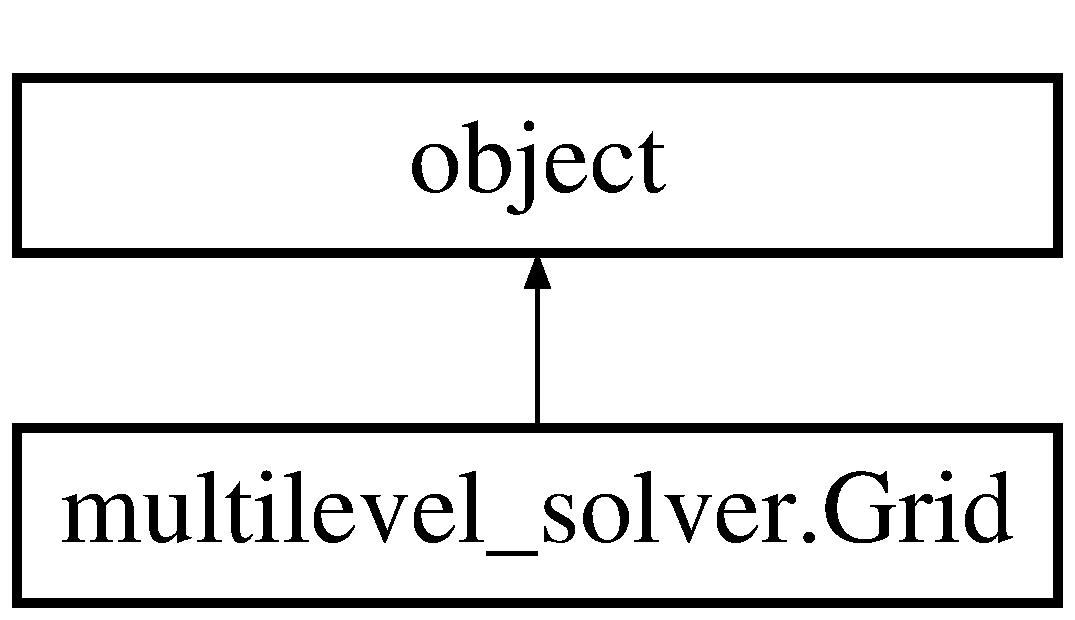
\includegraphics[height=2.000000cm]{classmultilevel__solver_1_1_grid}
\end{center}
\end{figure}
\subsection*{Public Member Functions}
\begin{DoxyCompactItemize}
\item 
def {\bf \+\_\+\+\_\+init\+\_\+\+\_\+} (self, T, S, phi, q)
\end{DoxyCompactItemize}
\subsection*{Public Attributes}
\begin{DoxyCompactItemize}
\item 
{\bfseries T}\label{classmultilevel__solver_1_1_grid_a0b7bf6fa097bf746b5184ab01cdcde5e}

\item 
{\bfseries S}\label{classmultilevel__solver_1_1_grid_a09afc3b3bff07c40e9be152c58ad76cf}

\item 
{\bfseries phi}\label{classmultilevel__solver_1_1_grid_a8af9e729a98a54799ec600de52bcfe6c}

\item 
{\bfseries q}\label{classmultilevel__solver_1_1_grid_a703241b145c02c58b2e8edb36ab3d2e6}

\end{DoxyCompactItemize}


\subsection{Detailed Description}
\begin{DoxyVerb}Grid class: simply makes a grid storing cross section, source, and moment data\end{DoxyVerb}
 

\subsection{Constructor \& Destructor Documentation}
\index{multilevel\+\_\+solver\+::\+Grid@{multilevel\+\_\+solver\+::\+Grid}!\+\_\+\+\_\+init\+\_\+\+\_\+@{\+\_\+\+\_\+init\+\_\+\+\_\+}}
\index{\+\_\+\+\_\+init\+\_\+\+\_\+@{\+\_\+\+\_\+init\+\_\+\+\_\+}!multilevel\+\_\+solver\+::\+Grid@{multilevel\+\_\+solver\+::\+Grid}}
\subsubsection[{\+\_\+\+\_\+init\+\_\+\+\_\+(self, T, S, phi, q)}]{\setlength{\rightskip}{0pt plus 5cm}def multilevel\+\_\+solver.\+Grid.\+\_\+\+\_\+init\+\_\+\+\_\+ (
\begin{DoxyParamCaption}
\item[{}]{self, }
\item[{}]{T, }
\item[{}]{S, }
\item[{}]{phi, }
\item[{}]{q}
\end{DoxyParamCaption}
)}\label{classmultilevel__solver_1_1_grid_aecd47351e8a88ac7c4b6d019d4083933}
\begin{DoxyVerb}Grid class: simply makes a grid storing cross section, source, and moment data\end{DoxyVerb}
 

The documentation for this class was generated from the following file\+:\begin{DoxyCompactItemize}
\item 
multilevel\+\_\+solver.\+py\end{DoxyCompactItemize}

\section{multilevel\+\_\+solver.\+Grid\+Set Class Reference}
\label{classmultilevel__solver_1_1_grid_set}\index{multilevel\+\_\+solver.\+Grid\+Set@{multilevel\+\_\+solver.\+Grid\+Set}}
Inheritance diagram for multilevel\+\_\+solver.\+Grid\+Set\+:\begin{figure}[H]
\begin{center}
\leavevmode
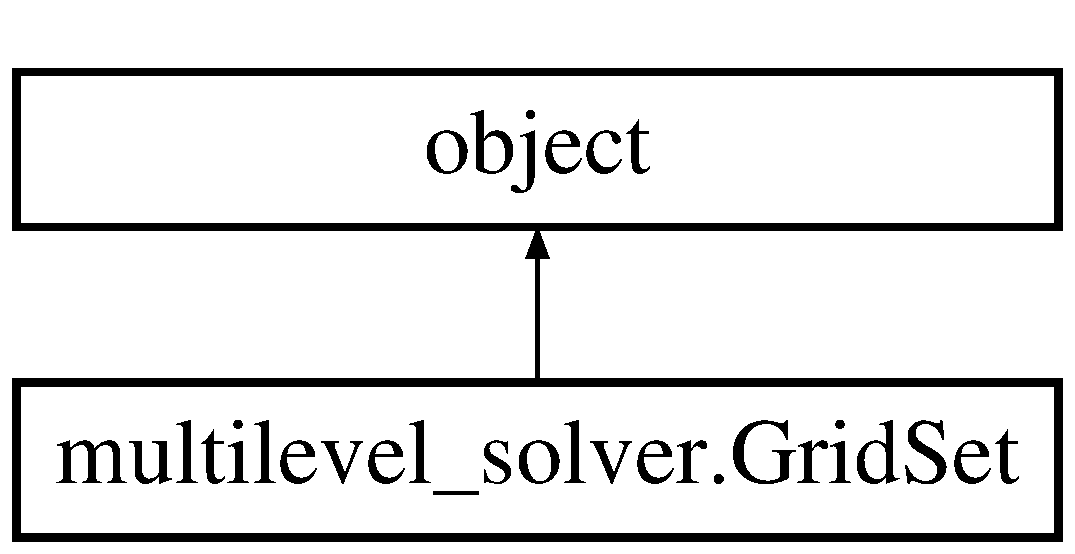
\includegraphics[height=2.000000cm]{classmultilevel__solver_1_1_grid_set}
\end{center}
\end{figure}
\subsection*{Public Member Functions}
\begin{DoxyCompactItemize}
\item 
def {\bfseries \+\_\+\+\_\+init\+\_\+\+\_\+} (self, G, H, {\bf phi}, q, Tname, Sname)\label{classmultilevel__solver_1_1_grid_set_ac67e7da7d78fd54e3a857877fc773244}

\item 
def {\bf prnt\+\_\+data} (self, level)
\item 
def {\bfseries relax} (self, nu, omega, level)\label{classmultilevel__solver_1_1_grid_set_a8421870f0278c6412b7894ecd9f1f25b}

\item 
def {\bf prolong} (self, data, level)
\item 
def {\bfseries restrict\+Mat} (self, data)\label{classmultilevel__solver_1_1_grid_set_af6c66f05d5e7e874b6e1b00a4958b1eb}

\item 
def {\bfseries restrict} (self, data)\label{classmultilevel__solver_1_1_grid_set_a0680fd0c22a8b46eed0f3d8de7af5488}

\item 
def {\bfseries residual} (self, level)\label{classmultilevel__solver_1_1_grid_set_a22f0050c0f960551869b255b2397f7a4}

\item 
def {\bfseries correct} (self, level)\label{classmultilevel__solver_1_1_grid_set_a5ed53041596e0d9185b14d0e3af1b2c9}

\item 
def {\bfseries direct} (self, level)\label{classmultilevel__solver_1_1_grid_set_a9c8925fc58196c7944cb068030dbd908}

\item 
def {\bfseries test\+\_\+convergence} (self, tol)\label{classmultilevel__solver_1_1_grid_set_ab90a9e459b5dcfbf9d2c3b8826e5e318}

\end{DoxyCompactItemize}
\subsection*{Static Public Attributes}
\begin{DoxyCompactItemize}
\item 
{\bf T} = np.\+zeros((G,G))
\item 
{\bfseries f} = open(Tname)\label{classmultilevel__solver_1_1_grid_set_a9b73b228e2dc3f229c46af67a8a210dc}

\item 
{\bfseries vals} = line.\+split()\label{classmultilevel__solver_1_1_grid_set_a772b384e433061bfbd1162b28aff7df4}

\item 
{\bfseries S} = np.\+zeros((G,G))\label{classmultilevel__solver_1_1_grid_set_a690ddac10746e324d51532fd07824319}

\item 
{\bfseries grids}\label{classmultilevel__solver_1_1_grid_set_a8a8cdecf798636c0bed2f0ad88f45527}

\item 
{\bfseries dtype}\label{classmultilevel__solver_1_1_grid_set_a1d55c1f48f205b92d1dea1b98b9183ef}

\item 
{\bfseries previous}\label{classmultilevel__solver_1_1_grid_set_ac2d3ae067871ce53d1808883982556e0}

\item 
{\bfseries init\+\_\+guess} = self.\+restrict(np.\+zeros(np.\+size(self.\+grids[level].{\bf T}, 0)))\label{classmultilevel__solver_1_1_grid_set_ae100d604c98077a706e062a9eb862809}

\item 
{\bfseries q} = self.\+grids[level].q\label{classmultilevel__solver_1_1_grid_set_afc3ace0ff6ed59d36d919f415409b0ac}

\item 
{\bfseries phi\+\_\+new} = copy.\+deepcopy(self.\+grids[level].{\bf phi})\label{classmultilevel__solver_1_1_grid_set_a9e069017c1cc277efe37814eef9b6ddf}

\item 
{\bfseries phi\+\_\+old} = copy.\+deepcopy(phi\+\_\+new)\label{classmultilevel__solver_1_1_grid_set_a6f5be1f719a27eecefc53ebd92201bb1}

\item 
int {\bfseries down} = 0\label{classmultilevel__solver_1_1_grid_set_a863767ce4b23e220555f25661f7fc0e0}

\item 
int {\bfseries up} = 0\label{classmultilevel__solver_1_1_grid_set_ad4617f2f8b0cbfe4f5af010fb18349f3}

\item 
{\bfseries down} = down+S[g, gp]$\ast$phi\+\_\+new[gp]\label{classmultilevel__solver_1_1_grid_set_ae1d95791d2c5e09e2b7f0f49698d695e}

\item 
{\bfseries up} = up+S[g, gp]$\ast$phi\+\_\+old[gp]\label{classmultilevel__solver_1_1_grid_set_a24c95a1ccdcf7527c1c9fc6af4eba572}

\item 
tuple {\bfseries D} = ({\bf T}[g, g] -\/ S[g, g])\label{classmultilevel__solver_1_1_grid_set_a343466da52e736f54da84240f7aa1d00}

\item 
{\bf phi}
\item 
{\bf num\+\_\+fine} = np.\+size(data,0)
\item 
int {\bfseries indx\+\_\+fine} = {\bf num\+\_\+fine}-\/1\label{classmultilevel__solver_1_1_grid_set_a0d14400f3187938c13fc4dc7e69bdc11}

\item 
{\bfseries indx\+\_\+coarse} = int(math.\+floor(indx\+\_\+fine/2))\label{classmultilevel__solver_1_1_grid_set_ac9130429945c3c362ed5f6b3486fd2d1}

\item 
int {\bfseries num\+\_\+coarse} = indx\+\_\+coarse+1\label{classmultilevel__solver_1_1_grid_set_a85786972d0474377aa1ec653457089b8}

\item 
{\bfseries data\+\_\+tmp} = np.\+zeros((num\+\_\+coarse, {\bf num\+\_\+fine}))\label{classmultilevel__solver_1_1_grid_set_ab8efbb954bd7e454df96d96ea4a62cb9}

\item 
{\bfseries data\+\_\+out} = np.\+zeros((num\+\_\+coarse, num\+\_\+coarse))\label{classmultilevel__solver_1_1_grid_set_a5cf175528e47b612c09baece04e354a4}

\item 
{\bf lhs} = np.\+dot((self.\+grids[level].{\bf T} -\/ self.\+grids[level].S), self.\+grids[level].{\bf phi})
\item 
{\bfseries r} = self.\+grids[level].q-\/{\bf lhs}\label{classmultilevel__solver_1_1_grid_set_ae0623319fb298cfa66f715bf4fd72f58}

\item 
{\bf correction} = self.\+prolong(self.\+grids[level].{\bf phi}, level)
\item 
{\bfseries corrected\+\_\+phi} = self.\+grids[level-\/1].{\bf phi}+{\bf correction}\label{classmultilevel__solver_1_1_grid_set_ae3a2829850e71626fa08b32f534eff1f}

\item 
{\bf error} = np.\+linalg.\+norm(self.\+previous -\/ self.\+grids[0].{\bf phi})
\end{DoxyCompactItemize}


\subsection{Detailed Description}
\begin{DoxyVerb}GridSet class: holds each grid, reads data, smooths, prolongs, and restricts\end{DoxyVerb}
 

\subsection{Member Function Documentation}
\index{multilevel\+\_\+solver\+::\+Grid\+Set@{multilevel\+\_\+solver\+::\+Grid\+Set}!prnt\+\_\+data@{prnt\+\_\+data}}
\index{prnt\+\_\+data@{prnt\+\_\+data}!multilevel\+\_\+solver\+::\+Grid\+Set@{multilevel\+\_\+solver\+::\+Grid\+Set}}
\subsubsection[{prnt\+\_\+data(self, level)}]{\setlength{\rightskip}{0pt plus 5cm}def multilevel\+\_\+solver.\+Grid\+Set.\+prnt\+\_\+data (
\begin{DoxyParamCaption}
\item[{}]{self, }
\item[{}]{level}
\end{DoxyParamCaption}
)}\label{classmultilevel__solver_1_1_grid_set_a2a35157a9be88e8a81f1a0bc61fcc523}
\begin{DoxyVerb}prnt_data: prints the value of phi for a given level\end{DoxyVerb}
 \index{multilevel\+\_\+solver\+::\+Grid\+Set@{multilevel\+\_\+solver\+::\+Grid\+Set}!prolong@{prolong}}
\index{prolong@{prolong}!multilevel\+\_\+solver\+::\+Grid\+Set@{multilevel\+\_\+solver\+::\+Grid\+Set}}
\subsubsection[{prolong(self, data, level)}]{\setlength{\rightskip}{0pt plus 5cm}def multilevel\+\_\+solver.\+Grid\+Set.\+prolong (
\begin{DoxyParamCaption}
\item[{}]{self, }
\item[{}]{data, }
\item[{}]{level}
\end{DoxyParamCaption}
)}\label{classmultilevel__solver_1_1_grid_set_a18c6c8b9b5bf4cdb36f51c5166b59ddf}
\begin{DoxyVerb}prolong: interpolates a vector from coarse to fine grids\end{DoxyVerb}
 

\subsection{Member Data Documentation}
\index{multilevel\+\_\+solver\+::\+Grid\+Set@{multilevel\+\_\+solver\+::\+Grid\+Set}!correction@{correction}}
\index{correction@{correction}!multilevel\+\_\+solver\+::\+Grid\+Set@{multilevel\+\_\+solver\+::\+Grid\+Set}}
\subsubsection[{correction}]{\setlength{\rightskip}{0pt plus 5cm}multilevel\+\_\+solver.\+Grid\+Set.\+correction = self.\+prolong(self.\+grids[level].{\bf phi}, level)\hspace{0.3cm}{\ttfamily [static]}}\label{classmultilevel__solver_1_1_grid_set_aae1405c5f4ea1b3d0a28f2bbbb1461fb}
\begin{DoxyVerb}correct: corrects and updates the solution on the previous level\end{DoxyVerb}
 \index{multilevel\+\_\+solver\+::\+Grid\+Set@{multilevel\+\_\+solver\+::\+Grid\+Set}!error@{error}}
\index{error@{error}!multilevel\+\_\+solver\+::\+Grid\+Set@{multilevel\+\_\+solver\+::\+Grid\+Set}}
\subsubsection[{error}]{\setlength{\rightskip}{0pt plus 5cm}multilevel\+\_\+solver.\+Grid\+Set.\+error = np.\+linalg.\+norm(self.\+previous -\/ self.\+grids[0].{\bf phi})\hspace{0.3cm}{\ttfamily [static]}}\label{classmultilevel__solver_1_1_grid_set_adf738b523c2cf33c3768c69040c380ef}
\begin{DoxyVerb}test_convergence: test if the system has converged\end{DoxyVerb}
 \index{multilevel\+\_\+solver\+::\+Grid\+Set@{multilevel\+\_\+solver\+::\+Grid\+Set}!lhs@{lhs}}
\index{lhs@{lhs}!multilevel\+\_\+solver\+::\+Grid\+Set@{multilevel\+\_\+solver\+::\+Grid\+Set}}
\subsubsection[{lhs}]{\setlength{\rightskip}{0pt plus 5cm}multilevel\+\_\+solver.\+Grid\+Set.\+lhs = np.\+dot((self.\+grids[level].{\bf T} -\/ self.\+grids[level].S), self.\+grids[level].{\bf phi})\hspace{0.3cm}{\ttfamily [static]}}\label{classmultilevel__solver_1_1_grid_set_aec4b52672b82fd48fb63078f6b05ed02}
\begin{DoxyVerb}residual: puts the residual into the next level source vector\end{DoxyVerb}
 \index{multilevel\+\_\+solver\+::\+Grid\+Set@{multilevel\+\_\+solver\+::\+Grid\+Set}!num\+\_\+fine@{num\+\_\+fine}}
\index{num\+\_\+fine@{num\+\_\+fine}!multilevel\+\_\+solver\+::\+Grid\+Set@{multilevel\+\_\+solver\+::\+Grid\+Set}}
\subsubsection[{num\+\_\+fine}]{\setlength{\rightskip}{0pt plus 5cm}multilevel\+\_\+solver.\+Grid\+Set.\+num\+\_\+fine = np.\+size(data,0)\hspace{0.3cm}{\ttfamily [static]}}\label{classmultilevel__solver_1_1_grid_set_aab6805fdddd81cb0bff39c74a1db5ebd}
\begin{DoxyVerb}restrictMat: restricts a matrix from fine to coarse grids\end{DoxyVerb}


\begin{DoxyVerb}restrict: restricts a vector from fine to coarse grids\end{DoxyVerb}
 \index{multilevel\+\_\+solver\+::\+Grid\+Set@{multilevel\+\_\+solver\+::\+Grid\+Set}!phi@{phi}}
\index{phi@{phi}!multilevel\+\_\+solver\+::\+Grid\+Set@{multilevel\+\_\+solver\+::\+Grid\+Set}}
\subsubsection[{phi}]{\setlength{\rightskip}{0pt plus 5cm}multilevel\+\_\+solver.\+Grid\+Set.\+phi\hspace{0.3cm}{\ttfamily [static]}}\label{classmultilevel__solver_1_1_grid_set_a89f4924177047261d47c0a17403fb4f7}
\begin{DoxyVerb}direct: directly solves the problem on the coarsest grid\end{DoxyVerb}
 \index{multilevel\+\_\+solver\+::\+Grid\+Set@{multilevel\+\_\+solver\+::\+Grid\+Set}!T@{T}}
\index{T@{T}!multilevel\+\_\+solver\+::\+Grid\+Set@{multilevel\+\_\+solver\+::\+Grid\+Set}}
\subsubsection[{T}]{\setlength{\rightskip}{0pt plus 5cm}multilevel\+\_\+solver.\+Grid\+Set.\+T = np.\+zeros((G,G))\hspace{0.3cm}{\ttfamily [static]}}\label{classmultilevel__solver_1_1_grid_set_aa463b40444b917ad445277651a853295}
\begin{DoxyVerb}relax: apply the iteration method\end{DoxyVerb}
 

The documentation for this class was generated from the following file\+:\begin{DoxyCompactItemize}
\item 
multilevel\+\_\+solver.\+py\end{DoxyCompactItemize}

\section{Est\+Num\+Jellies.\+Num\+Jelly\+Estimator Class Reference}
\label{class_est_num_jellies_1_1_num_jelly_estimator}\index{Est\+Num\+Jellies.\+Num\+Jelly\+Estimator@{Est\+Num\+Jellies.\+Num\+Jelly\+Estimator}}


This class estimates the number of jelly beans in the world using input data determined to be correlated to this result.  


\subsection*{Public Member Functions}
\begin{DoxyCompactItemize}
\item 
def {\bf \+\_\+\+\_\+init\+\_\+\+\_\+} (self)
\begin{DoxyCompactList}\small\item\em Instantiating the class initializes some variables. \end{DoxyCompactList}\item 
def {\bf set\+\_\+land\+\_\+frac\+\_\+for\+\_\+sugar} (self, frac)
\begin{DoxyCompactList}\small\item\em Set the fraction of land used for sugar. \end{DoxyCompactList}\item 
def {\bf set\+\_\+world\+\_\+pop} (self, people)
\begin{DoxyCompactList}\small\item\em Set the world population. \end{DoxyCompactList}\item 
def {\bf set\+\_\+frac\+\_\+ppl\+\_\+loving\+\_\+pink} (self, frac)
\begin{DoxyCompactList}\small\item\em Set the fraction of people who love the color pink. \end{DoxyCompactList}\item 
def {\bf get\+\_\+scaling\+\_\+const} (self)
\begin{DoxyCompactList}\small\item\em Return the scaling constant so the user can check it if they want. \end{DoxyCompactList}\item 
def {\bf compute\+\_\+\+Njelly\+\_\+est} (self)
\begin{DoxyCompactList}\small\item\em Estimate the number of jelly beans in the world. \end{DoxyCompactList}\item 
def {\bf compute\+\_\+\+Njelly\+\_\+pink\+\_\+est} (self)
\begin{DoxyCompactList}\small\item\em Estimate the number of jelly beans in the world using new data, regarding the fraction of people in the world who love the color pink. \end{DoxyCompactList}\end{DoxyCompactItemize}
\subsection*{Public Attributes}
\begin{DoxyCompactItemize}
\item 
{\bf frac\+Land4\+Sugar}\label{class_est_num_jellies_1_1_num_jelly_estimator_a9718c54b9d7b610eb5789852daff3661}

\begin{DoxyCompactList}\small\item\em Fraction of land used for growing sugar. \end{DoxyCompactList}\item 
{\bf world\+Pop}\label{class_est_num_jellies_1_1_num_jelly_estimator_afcc81dee96f41bbac3b8a798bcc9a525}

\begin{DoxyCompactList}\small\item\em World population. \end{DoxyCompactList}\item 
{\bf scaling\+Const}\label{class_est_num_jellies_1_1_num_jelly_estimator_a4eef3f82cd4820f723b878333c21f9ce}

\begin{DoxyCompactList}\small\item\em Scaling constant used in estimate. \end{DoxyCompactList}\item 
{\bf frac\+Ppl\+Loving\+Pink}
\begin{DoxyCompactList}\small\item\em Fraction of people who love the color pink. \end{DoxyCompactList}\end{DoxyCompactItemize}


\subsection{Detailed Description}
This class estimates the number of jelly beans in the world using input data determined to be correlated to this result. 

The number of jelly beans in the world is correlated to the fraction of land used for sugar, the world population, and the fraction of people who like the color pink. 

\subsection{Constructor \& Destructor Documentation}
\index{Est\+Num\+Jellies\+::\+Num\+Jelly\+Estimator@{Est\+Num\+Jellies\+::\+Num\+Jelly\+Estimator}!\+\_\+\+\_\+init\+\_\+\+\_\+@{\+\_\+\+\_\+init\+\_\+\+\_\+}}
\index{\+\_\+\+\_\+init\+\_\+\+\_\+@{\+\_\+\+\_\+init\+\_\+\+\_\+}!Est\+Num\+Jellies\+::\+Num\+Jelly\+Estimator@{Est\+Num\+Jellies\+::\+Num\+Jelly\+Estimator}}
\subsubsection[{\+\_\+\+\_\+init\+\_\+\+\_\+(self)}]{\setlength{\rightskip}{0pt plus 5cm}def Est\+Num\+Jellies.\+Num\+Jelly\+Estimator.\+\_\+\+\_\+init\+\_\+\+\_\+ (
\begin{DoxyParamCaption}
\item[{}]{self}
\end{DoxyParamCaption}
)}\label{class_est_num_jellies_1_1_num_jelly_estimator_ab5d187b2dfbd0a52034edc88a6cd9171}


Instantiating the class initializes some variables. 



\subsection{Member Function Documentation}
\index{Est\+Num\+Jellies\+::\+Num\+Jelly\+Estimator@{Est\+Num\+Jellies\+::\+Num\+Jelly\+Estimator}!compute\+\_\+\+Njelly\+\_\+est@{compute\+\_\+\+Njelly\+\_\+est}}
\index{compute\+\_\+\+Njelly\+\_\+est@{compute\+\_\+\+Njelly\+\_\+est}!Est\+Num\+Jellies\+::\+Num\+Jelly\+Estimator@{Est\+Num\+Jellies\+::\+Num\+Jelly\+Estimator}}
\subsubsection[{compute\+\_\+\+Njelly\+\_\+est(self)}]{\setlength{\rightskip}{0pt plus 5cm}def Est\+Num\+Jellies.\+Num\+Jelly\+Estimator.\+compute\+\_\+\+Njelly\+\_\+est (
\begin{DoxyParamCaption}
\item[{}]{self}
\end{DoxyParamCaption}
)}\label{class_est_num_jellies_1_1_num_jelly_estimator_ab4f98f6a7600e03ebea6fe738588c483}


Estimate the number of jelly beans in the world. 

This is based on a previous understanding of the estimate that did not take the color pink into account. Still supported for legacy reasons. \index{Est\+Num\+Jellies\+::\+Num\+Jelly\+Estimator@{Est\+Num\+Jellies\+::\+Num\+Jelly\+Estimator}!compute\+\_\+\+Njelly\+\_\+pink\+\_\+est@{compute\+\_\+\+Njelly\+\_\+pink\+\_\+est}}
\index{compute\+\_\+\+Njelly\+\_\+pink\+\_\+est@{compute\+\_\+\+Njelly\+\_\+pink\+\_\+est}!Est\+Num\+Jellies\+::\+Num\+Jelly\+Estimator@{Est\+Num\+Jellies\+::\+Num\+Jelly\+Estimator}}
\subsubsection[{compute\+\_\+\+Njelly\+\_\+pink\+\_\+est(self)}]{\setlength{\rightskip}{0pt plus 5cm}def Est\+Num\+Jellies.\+Num\+Jelly\+Estimator.\+compute\+\_\+\+Njelly\+\_\+pink\+\_\+est (
\begin{DoxyParamCaption}
\item[{}]{self}
\end{DoxyParamCaption}
)}\label{class_est_num_jellies_1_1_num_jelly_estimator_a5a4f72a37cd411a42b24c9621c436a01}


Estimate the number of jelly beans in the world using new data, regarding the fraction of people in the world who love the color pink. 

\index{Est\+Num\+Jellies\+::\+Num\+Jelly\+Estimator@{Est\+Num\+Jellies\+::\+Num\+Jelly\+Estimator}!get\+\_\+scaling\+\_\+const@{get\+\_\+scaling\+\_\+const}}
\index{get\+\_\+scaling\+\_\+const@{get\+\_\+scaling\+\_\+const}!Est\+Num\+Jellies\+::\+Num\+Jelly\+Estimator@{Est\+Num\+Jellies\+::\+Num\+Jelly\+Estimator}}
\subsubsection[{get\+\_\+scaling\+\_\+const(self)}]{\setlength{\rightskip}{0pt plus 5cm}def Est\+Num\+Jellies.\+Num\+Jelly\+Estimator.\+get\+\_\+scaling\+\_\+const (
\begin{DoxyParamCaption}
\item[{}]{self}
\end{DoxyParamCaption}
)}\label{class_est_num_jellies_1_1_num_jelly_estimator_a8cc61de7181d21d6c1da52ddc1e7d133}


Return the scaling constant so the user can check it if they want. 

\index{Est\+Num\+Jellies\+::\+Num\+Jelly\+Estimator@{Est\+Num\+Jellies\+::\+Num\+Jelly\+Estimator}!set\+\_\+frac\+\_\+ppl\+\_\+loving\+\_\+pink@{set\+\_\+frac\+\_\+ppl\+\_\+loving\+\_\+pink}}
\index{set\+\_\+frac\+\_\+ppl\+\_\+loving\+\_\+pink@{set\+\_\+frac\+\_\+ppl\+\_\+loving\+\_\+pink}!Est\+Num\+Jellies\+::\+Num\+Jelly\+Estimator@{Est\+Num\+Jellies\+::\+Num\+Jelly\+Estimator}}
\subsubsection[{set\+\_\+frac\+\_\+ppl\+\_\+loving\+\_\+pink(self, frac)}]{\setlength{\rightskip}{0pt plus 5cm}def Est\+Num\+Jellies.\+Num\+Jelly\+Estimator.\+set\+\_\+frac\+\_\+ppl\+\_\+loving\+\_\+pink (
\begin{DoxyParamCaption}
\item[{}]{self, }
\item[{}]{frac}
\end{DoxyParamCaption}
)}\label{class_est_num_jellies_1_1_num_jelly_estimator_a3af6f81c95c3b551174d39509615cb0e}


Set the fraction of people who love the color pink. 


\begin{DoxyParams}{Parameters}
{\em people} & integer number of people who love the color pink \\
\hline
\end{DoxyParams}
\index{Est\+Num\+Jellies\+::\+Num\+Jelly\+Estimator@{Est\+Num\+Jellies\+::\+Num\+Jelly\+Estimator}!set\+\_\+land\+\_\+frac\+\_\+for\+\_\+sugar@{set\+\_\+land\+\_\+frac\+\_\+for\+\_\+sugar}}
\index{set\+\_\+land\+\_\+frac\+\_\+for\+\_\+sugar@{set\+\_\+land\+\_\+frac\+\_\+for\+\_\+sugar}!Est\+Num\+Jellies\+::\+Num\+Jelly\+Estimator@{Est\+Num\+Jellies\+::\+Num\+Jelly\+Estimator}}
\subsubsection[{set\+\_\+land\+\_\+frac\+\_\+for\+\_\+sugar(self, frac)}]{\setlength{\rightskip}{0pt plus 5cm}def Est\+Num\+Jellies.\+Num\+Jelly\+Estimator.\+set\+\_\+land\+\_\+frac\+\_\+for\+\_\+sugar (
\begin{DoxyParamCaption}
\item[{}]{self, }
\item[{}]{frac}
\end{DoxyParamCaption}
)}\label{class_est_num_jellies_1_1_num_jelly_estimator_a2f42a6d687f98d5128983ff43d6b4989}


Set the fraction of land used for sugar. 


\begin{DoxyParams}{Parameters}
{\em frac} & fraction of land used for sugar (float between 0 and 1) \\
\hline
\end{DoxyParams}
\index{Est\+Num\+Jellies\+::\+Num\+Jelly\+Estimator@{Est\+Num\+Jellies\+::\+Num\+Jelly\+Estimator}!set\+\_\+world\+\_\+pop@{set\+\_\+world\+\_\+pop}}
\index{set\+\_\+world\+\_\+pop@{set\+\_\+world\+\_\+pop}!Est\+Num\+Jellies\+::\+Num\+Jelly\+Estimator@{Est\+Num\+Jellies\+::\+Num\+Jelly\+Estimator}}
\subsubsection[{set\+\_\+world\+\_\+pop(self, people)}]{\setlength{\rightskip}{0pt plus 5cm}def Est\+Num\+Jellies.\+Num\+Jelly\+Estimator.\+set\+\_\+world\+\_\+pop (
\begin{DoxyParamCaption}
\item[{}]{self, }
\item[{}]{people}
\end{DoxyParamCaption}
)}\label{class_est_num_jellies_1_1_num_jelly_estimator_a0244b2d3252a7b1d7106fae186121d75}


Set the world population. 


\begin{DoxyParams}{Parameters}
{\em people} & integer number of people on earth \\
\hline
\end{DoxyParams}


\subsection{Member Data Documentation}
\index{Est\+Num\+Jellies\+::\+Num\+Jelly\+Estimator@{Est\+Num\+Jellies\+::\+Num\+Jelly\+Estimator}!frac\+Ppl\+Loving\+Pink@{frac\+Ppl\+Loving\+Pink}}
\index{frac\+Ppl\+Loving\+Pink@{frac\+Ppl\+Loving\+Pink}!Est\+Num\+Jellies\+::\+Num\+Jelly\+Estimator@{Est\+Num\+Jellies\+::\+Num\+Jelly\+Estimator}}
\subsubsection[{frac\+Ppl\+Loving\+Pink}]{\setlength{\rightskip}{0pt plus 5cm}Est\+Num\+Jellies.\+Num\+Jelly\+Estimator.\+frac\+Ppl\+Loving\+Pink}\label{class_est_num_jellies_1_1_num_jelly_estimator_adf6fe4e805106a7316b3202cc5c3470e}


Fraction of people who love the color pink. 



The documentation for this class was generated from the following file\+:\begin{DoxyCompactItemize}
\item 
Est\+Num\+Jellies.\+py\end{DoxyCompactItemize}

%--- End generated contents ---

% Index
\backmatter
\newpage
\phantomsection
\clearemptydoublepage
\addcontentsline{toc}{chapter}{Index}
\printindex

\end{document}
